\documentclass[11pt]{beamer}
\mode<article> % only for the article version
{
  \usepackage{fullpage}
  \usepackage{hyperref}
%\usepackage[ps2pdf]{hyperref}
}
\usepackage{epsfig}
\usepackage{fancybox}
\usefonttheme[onlymath]{serif}

\mode<presentation>
{
%  \setbeamertemplate{background canvas}[vertical shading][bottom=white,top=blue!10]
%     \usetheme{Warsaw}
% \usetheme{CambridgeUS}
%  	\usetheme{Frankfurt}
%  	\usetheme{Berlin}
%  	\usetheme{Antibes}
%   \usetheme{Darmstadt}
%    \usetheme{Madrid}
%    \usefonttheme[onlysmall]{structurebold}
 	\usecolortheme{orchid}
% 	\usecolortheme{seahorse}
  \usecolortheme[named=blue]{structure}
% 	\usecolortheme{crane}
%	\usecolortheme{lily}
}

\setbeamercolor{math text}{fg=green!50!black}
\setbeamercolor{normal text in math text}{parent=math text}

\usepackage{color}
\usepackage{epsfig}
\usepackage{amsmath}
\usepackage{amssymb}
%\usepackage{beamerthemesplit}
\usepackage{listings}
 \lstset{language=Python,
    basicstyle=\ttfamily\bfseries,
    commentstyle=\color{red}\itshape,
  stringstyle=\color{green},
  showstringspaces=false,
  keywordstyle=\color{blue}\bfseries,
  breaklines=true,
%  postbreak=\mbox{\textcolor{red}{$\hookrightarrow$}\space},
  }
  
\usepackage[vlined,algoruled,titlenotnumbered,linesnumbered]{algorithm2e}
\usepackage{color}
\newcommand{\argmaxF}{\mathop{\mathrm{argmax}}\limits}


%\usepackage{lmodern}
%\usepackage[T1]{fontenc} 

\setlength{\leftmargini}{0pt}

\usepackage{times}

\setbeamercovered{dynamic}

\title[NLP]{Natural Language Processing}
\subtitle{Lecture V. N-gram Language Models and TF-IDF}
\author[Forrest Sheng Bao]{Forrest Sheng Bao, Ph.D.}
\institute[ISU]{Dept. of Computer Science \\ Iowa State University \\ Ames, IA 50011}
\date[9/14/2021]{Sept. 14, 2021}

%\AtBeginSection[] {
%  \begin{frame}[plain]
%    \frametitle{Outline}
%    \tableofcontents[currentsection]
%  \end{frame}
%  \addtocounter{framenumber}{-1}
%}

\AtBeginSubsection[] {
  \begin{frame}[plain]
   \frametitle{Outline}
    \tableofcontents[currentsubsection]
    \addtocounter{framenumber}{-1}
  \end{frame}
} 

\begin{document}

 \frame{\titlepage}
 
 \section<presentation>*{Outline}
 
   \begin{frame}
     \frametitle{Outline}
  \tableofcontents
   \end{frame}

 
\section{Why language models}

\begin{frame}{Why language models}
For many applications, the output is a sequence of words.
 \begin{itemize}[<+->]
   \item Example 1: Machine translation (MT): 
   
\begin{center}
  \textit{ Sprechen Sie MATLAB?}  $\Rightarrow$ Do you speak MATLAB? 
\end{center}

\item Example 2: Automatic Speech Recognition (ASR): 
   
\hskip -5em
   \includegraphics[width=.5\textwidth]{random.pdf}  
   $\Rightarrow$
   ``\$2M seed from Sequoia?''
   \item Example 3: Spell checking or spell suggestion 
   
   
   \begin{center}
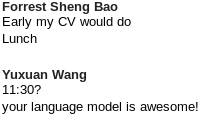
\includegraphics[width=.3\textwidth]{lunch.png}~~~~~~
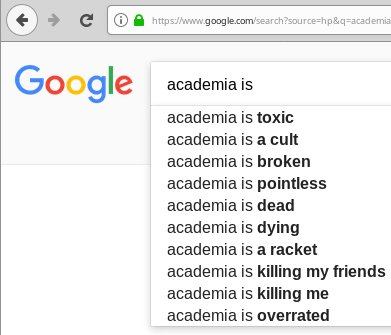
\includegraphics[width=.3\textwidth]{academia_is.png}
\end{center}     
   
 \item The system needs to evaluate/rank a set of candidates, e.g., ``\$2M seed from Sequoia?'' over ``\$2M seed from DFJ!''
 \item An easy way is to compute the likelihood that a candidate is a ``making-sense'' sentence. 
 \end{itemize}
\end{frame}

\begin{frame}{Ranking candidate text strings}
  \begin{itemize}
    \item For example, we can compute a probability for each string below: 
    \item S1: ``Please CALL me in 10 minutes.''
    \item S2: ``Please ALL me in 10 minutes.''
    \item Which one is bigger? $P(S_1)$ or $P(S_2)$?
  \end{itemize}
  
\end{frame}


\section{Language models }
\begin{frame}[shrink]{Language models}
\begin{itemize}[<+->]
 \item A statistical language model is a probability distribution over sequences of words. 
 \item Given a length $l$, a language model assigns a probability $P(w_1, \dots, w_l)$ to the sequence. 
 \item When $l=1$, we have the probability for each individual word. 
 \item When $l=2$, we have the probability for each two-word pair. 
 \item ...
 \item In the example above, the system will compare the probabilities $P(w_1=\text{``\$2M''}, w_2=\text{``seed''},  w_3=\text{``from''}, w_3= \text{``Sequoia''})$ and 
 $P(w_1= \text{``\$2M''}, w_2=\text{``seed''}, w_3= \text{``from''}, w_4=\text{``DFJ''})$. 
 \item By chain rule,  we have
 \begin{align*}
 & P(w_0=\rhd, w_1=\text{``\$2M''}, w_2=\text{``seed''}, w_3=\text{``from''}, w_4= \text{``Sequoia''}, w_5=\lhd) \\
 =  & 
P(w_1= \text{``\$2M''} | w_0= \rhd) \\
 \times &  P(w_2=\text{``seed''} | w_1= \text{``\$2M''}, w_0=\rhd) \\
 \times & P(w_3=\text{``from''} | w_2=\text{``seed''}, w_1= \text{``\$2M''}, w_0=\rhd) \\
 \times &  P(w_4= \text{``Sequoia''} | w_3=\text{``from''} , w_2=\text{``seed''}, w_1= \text{``\$2M''}, w_0=\rhd) \\
 \times & P(w_5= \lhd | w_4= \text{``Sequoia''}, w_3=\text{``from''} , w_2=\text{``seed''}, w_1= \text{``\$2M''}, w_0=\rhd)
 \end{align*}
 %  \item skip-gram: the probability for every the other words, e.g., ``natural processing'', ``langauge is'', ``processing a'', etc., from the sentence ``natural language processing is a study of computer science.''
 \end{itemize}
\end{frame}

\section{n-gram models}

\begin{frame}{n-gram models}
\begin{itemize}[<+->]
 \item Let's generalize: $P(w_1, \cdots, w_l) = \prod\limits_{i=1}^l P(w_i | w_1, \dots, w_{i-1})$
 \item Use a shorter history ($n$-th order Markov property): $\prod\limits_{i=1}^l P(w_i | w_1, \dots, w_{i-1}) \approx \prod\limits^l_{i=1} P(w_i\mid w_{i-(n-1)},\ldots,w_{i-1})$
 \item Conditional probability from counting: $P(w_i\mid w_{i-(n-1)},\ldots,w_{i-1}) = \frac{\mathrm{count}(w_{i-(n-1)},\ldots,w_{i-1},w_i)}{\mathrm{count}(w_{i-(n-1)},\ldots,w_{i-1})}$
%  \item The probability of observing the $i$-th word $w_i$ is approximately 
 \item When $n=1$, 2 or 3, it's unigram, bi-gram or tri-gram respectively. 
 \item Yes, unigram means no history but just the word itself. No order between words is considered. 
 \item N-gram is one (simple but widely used) way to represent language models. 
\end{itemize}
\end{frame}

\begin{frame}{Bag of words}
\begin{columns}
  \begin{column}{0.6\textwidth}
 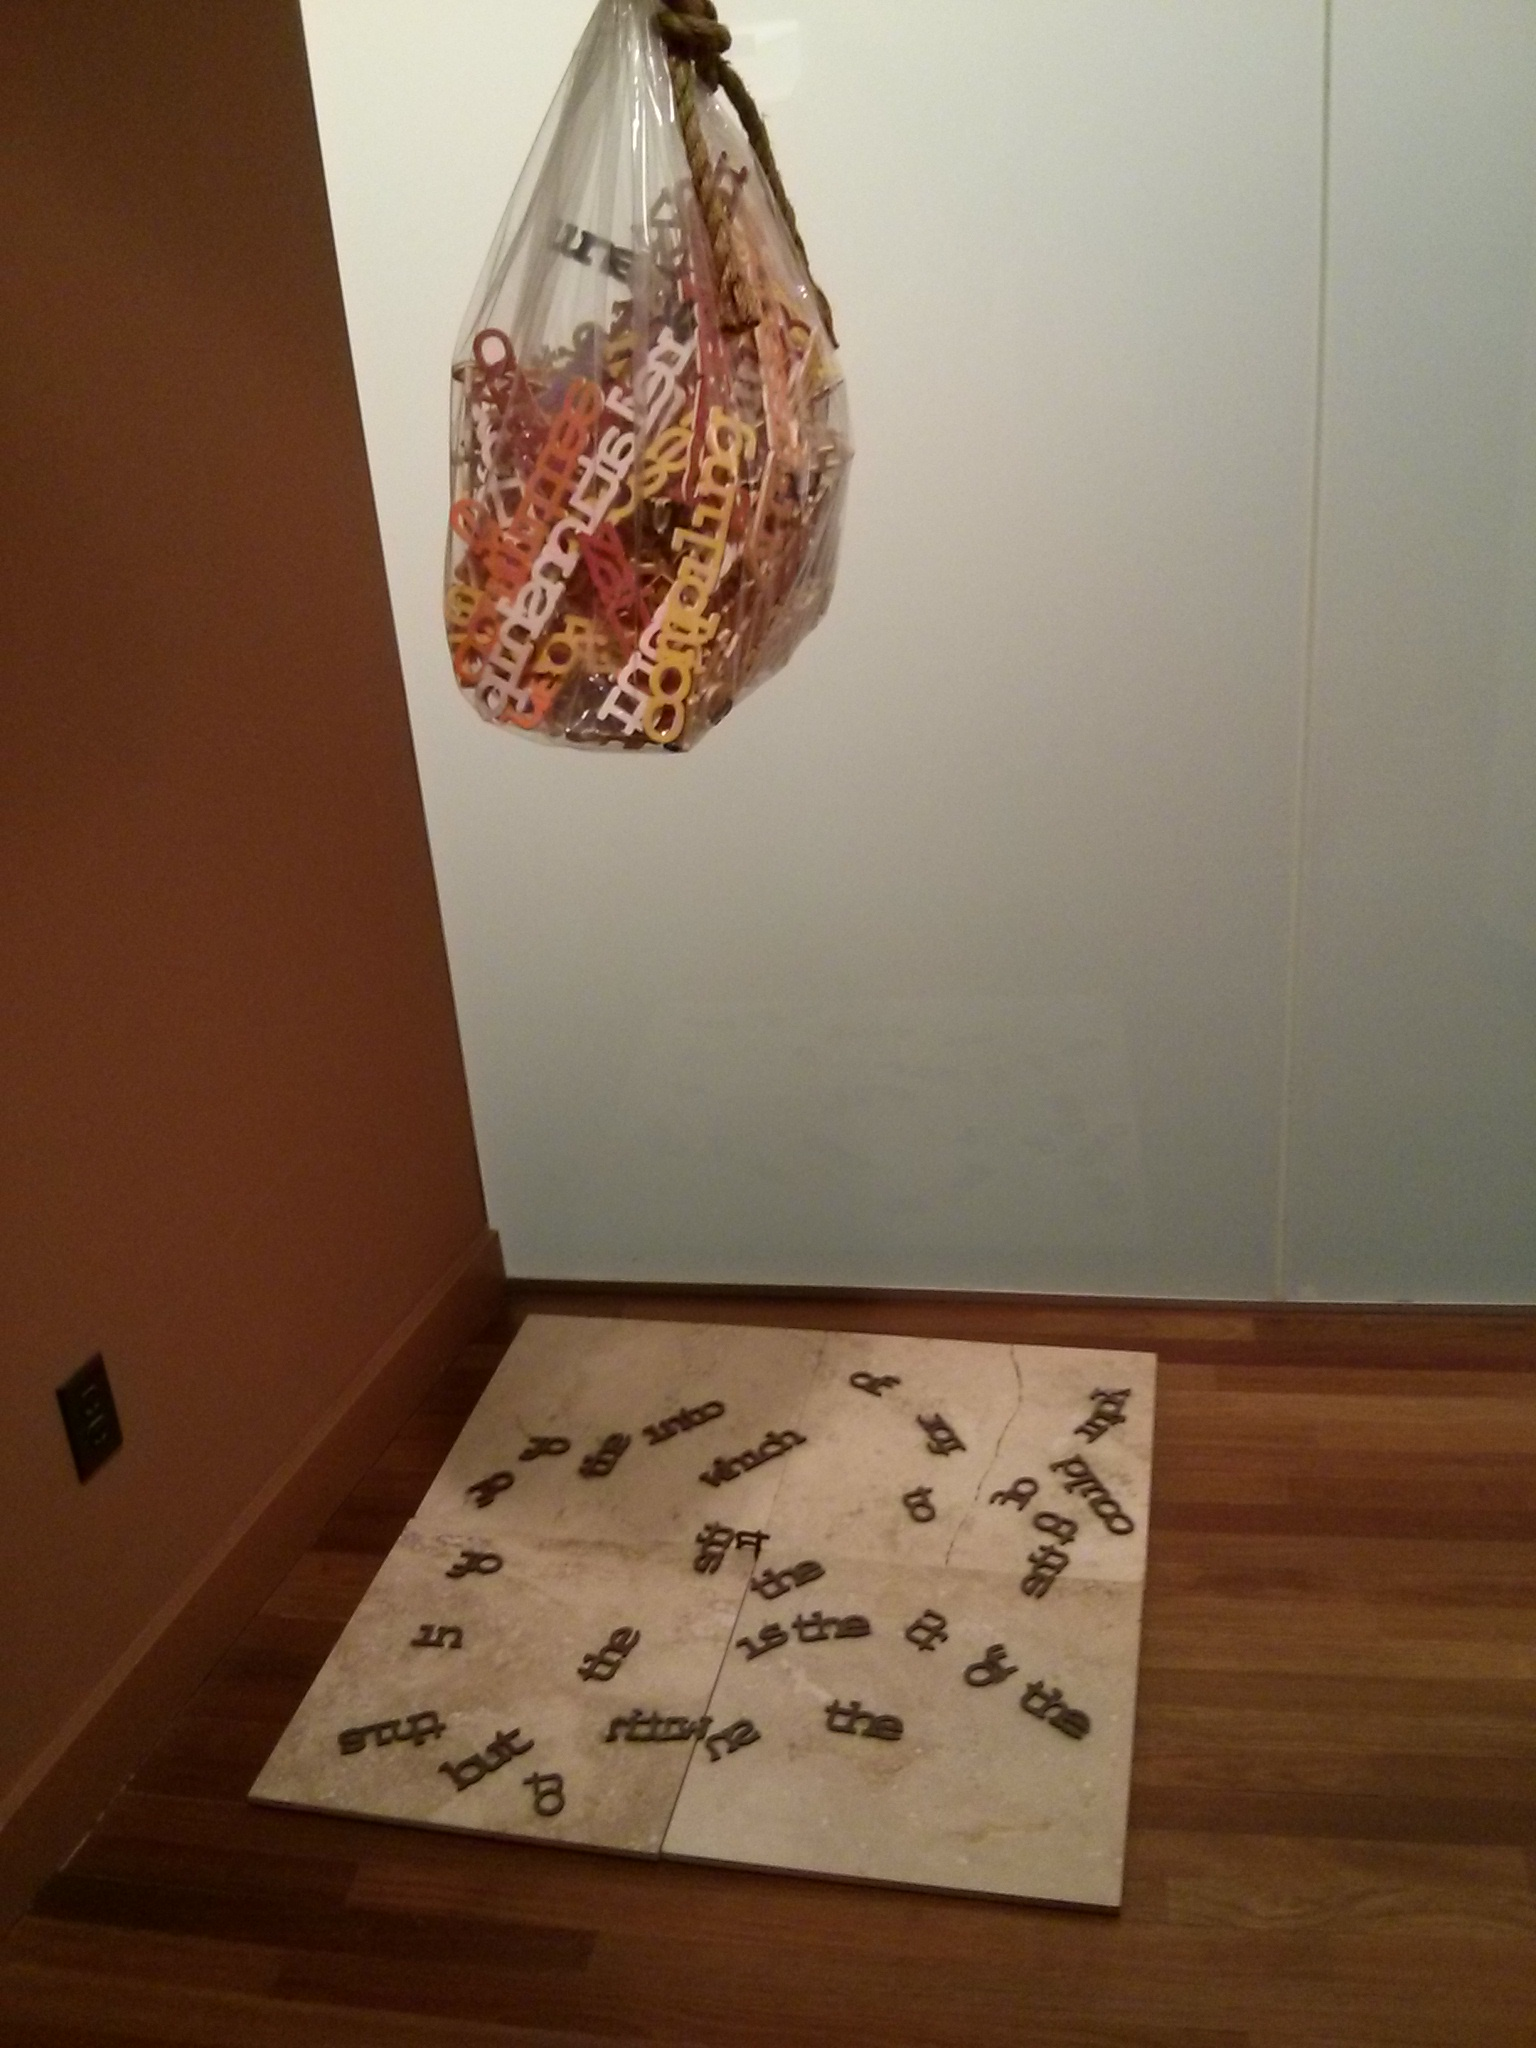
\includegraphics[width=\textwidth]{CMU_BOW.jpg}  
  \end{column}
 \begin{column}{0.5\textwidth}
 The bag of words and the background words as seen in Gates building, CMU
 \end{column}
\end{columns}
\end{frame}

\begin{frame}{Bag of words (cont.)}
 \begin{itemize}[<+->]
  \item A bag-of-words (BOW) model is basically a uni-gram model: an orderless representation of a document. 
  \item A common use of a BOW model is create feature vectors using the frequencies of words, i.e., term frequency. 
  \item Background words are those of extreme high frequency. They are earlier called stop words. 
  \item When many researchers use the term ``bigram'' or ``trigram'', they are actually talking about bag-of-double-words or bag-of-triple-words. 
  \item See \url{https://en.wikipedia.org/wiki/Bag-of-words_model}.
  \item Also, how to build a spam filter using BOW: \url{https://en.wikipedia.org/wiki/Naive_Bayes_spam_filtering}
 \end{itemize}
\end{frame}

\begin{frame}{skip-grams and CBOW}
 \begin{itemize}[<+->]
  \item We may also add a gap between words. 
  \item 1-degree Skip-grams from the sentence ``I am a PhD student'':
  
  (``I'', ``a''), (``am'', ``PhD''), (``a'', ``student''). 
  \item A language model using skip-gram:  
 $$P(w_{i} | w_{i-k}, \dots, w_{i-1},~~~~~, w_{i+1}, \dots, w_{i+k})$$
  \item NOT THE CASE! 
  \item Instead of estimating the probability giving the neighboring words, a skip-gram language model actually estimates the probabilities of neighboring words given a word: 
  \item $$\sum_{j\in[-k..-1]\cup [1..k]} \log P(w_{i+j} | w_i)$$
  \item The first equation is actually called Continues BOW (CBOW) model. 
 \end{itemize}
\end{frame}

\begin{frame}{Order of n-grams and interpolation}
 \begin{itemize}[<+->]
  \item Larger $n$: the string is specific but sparse, e.g., ``academia is vicious'' may not be in training data.
  \item Smaller $n$: dense but general, e.g., lots of ``academia is'' or maybe ``is vicious''
  \item To balance, mix different orders by interpolation: 
  $$\lambda_3 P(w_i|w_{i-1}, w_{i-2}) + \lambda_2 P(w_i|w_{i-1}) + \lambda_1 P(w_i)$$
  \item The challenge is how to choose weights. Many people use brutal force. 
  \item Better methods to be presented later. 
 \end{itemize}
\end{frame}

\section{Smoothing and Discounting}

\begin{frame}{Smoothing}
 \begin{itemize}[<+->]
  \item What about unknown words? 
  \item The problem is known as OOV (out of vocabulary)
  \item Lazy way: ignore them -- closed vocabulary. 
  \item For uni-gram: $$P_{\text{smoothed}} (w_i) = \lambda P_{\text{model}}(w_i) + (1-\lambda) \frac{1}{N},$$ where 
  \begin{itemize}
   \item   $N$ is the number of total vocabulary, 
   \item $\lambda$ is the probability that a word is known to the model (it can be totally arbitrary, e.g., $0.95$), 
   \item $P_{\text{model}}(w_i)$ is the probability of the word in a unigram model (thus, 0 if the word is not in the model). 
  \end{itemize}
  \item It means that all unknown words have the equal probability $\frac{1-\lambda}{N}$. 
 \end{itemize}
\end{frame}

\begin{frame}{Smoothing for bi-grams}
 \begin{itemize}[<+->]
  \item Observation: some words have more words following it while others have fewer. 
  \item Make the smoothing depend on the context, i.e., $\lambda$ is not the same for all words. 
  \item Also leverages the unigram model, i.e., interpolation. 
  \item $P_{\text{smoothed}}(w_i|w_{i-1}) = \lambda_{w_{i-1}} P_{\text{model}}(w_i|w_{i-1}) + (1-\lambda_{w_{i-1}})P_{\text{model}}(w_i)$
  \item Witten-Bell smoothing: $$\lambda_{w_{i-1}} = \frac{c(w_{i-1})}{u(w_{i-1}) + c(w_{i-1})}$$ where 
  $u(w_{i-1})$ is the number of unique words after $w_{i-1}$ and $c(w_{i-1})$ the total count of $w_{i-1}$ in the training corpus. 
 \end{itemize}
\end{frame}

% \begin{frame}{Discounting}
% \begin{itemize}
%  \item The unknown words (including unknown double-words, triple-words, etc.) introduces sparsity issue to n-gram models. 
% \end{itemize}
% \end{frame}

\begin{frame}{Evaluating a language model}
 \begin{itemize}[<+->]
  \item Likelihood: Given a test set $W_{test}$, compute the score $\prod\limits_{\mathbf{w}\in W_{test}} P(\mathbf{w} |M)$ where $M$ is the model and $\mathbf{w}$ is a sequence of words. 
  \item Example: Let $W_{test} = \{ \text{``I am a Linuxer''}, \text{``I am an entreprenuer''}, \text{``I am a Pythonista''}\}$. The score is $P(\text{``I am a Linuxer''}) \times P( \text{``I am an entreprenuer''}) \times  P( \text{``I am a Pythonista''}) $
  \item But, what if the model covers some sentences very well but not others? 
  \item Entropy
  \item And, coverage. 
 \end{itemize}
\end{frame}

\begin{frame}{Other language models}
Other ways to estimate $P(w_1, \dots, w_l)$ beyond n-gram: 
\begin{itemize}
 \item Exponential language models: maximum entropy language models, log-bilinear language models. 
 \item neural language models: based on neural networks, embedding 
\end{itemize}
\end{frame}

\section{Na\"ive Bayes spam filter}
\begin{frame}{Na\"ive Bayes spam filter}
  \begin{itemize}[<+->]
    \item A classical application of the BOW model
    \item Two classes: Spam ($S$) vs ham ($H$, non-spam)
    \item Based on Bayes theorem, given one word $w$, the chances that a message is spam: 
      $P(S|w)={P(S, w)\over P(w)} = { P(w|S)P(S) \over P(w|H)P(H)+P(w|S)P(S)} $
    \item Usually we further assume that $P(H)=P(S)$. Thus $P(S|w)= { P(w|S) \over P(w|H)+P(w|S)}$. Takeaway: all you need is $P(w|H)$ and $P(w|S)$ which can be obtained via counting. 
    % \item Independent events:  $P(A, B) = P(A|B)P(B) \text{~~or~~} P(B|A)P(A) =  P(A)\cdot P(B)$
    \item Na\"ive Bayes spam filters assume that  words appear in an email indepdently. So for two independent words $w_1$ and $w_2$ (not necessarily sequential), we have: 
%  $P(S|w_1, w_2)={P(S, w_1, w_2)\over P(w_1,w_2)} = {  P(w_2| w_1, S)P(w_1|S)P(S) \over \Pi_{i=1}^{2} \left [ P(w_i|H)P(H)+P(w_i|S)P(S)\right ] } = {  P(w_2| w_1, S) P(w_2|S)   P(w_1|S)P(S) \over \Pi_{i=1}^{2} \left [ P(w_i|H)P(H)+P(w_i|S)P(S)\right ] } $
 $P(S|w_1, w_2)={P(w_1|S) P(w_2|S) \over P(w_1|S) P(w_2|S) + (1-P(w_1|S)) (1- P(w_2|S))}$ 
 \item Detailed derivation at \url{http://www.paulgraham.com/naivebayes.html} and \url{https://www.mathpages.com/home/kmath267/kmath267.htm}

  \end{itemize}
  
\end{frame}


\section{TF-IDF}
\begin{frame}{TF-IDF}
  \begin{itemize}[<+->]
  \item How to create a feature vector to detect sentences about a topic? 
  \item Given a search term, e.g.,  ``matlab'', and a bunch of documents,  how to rank all documents that match the query? 
  \item Intuition 1: If a document has lots occurences of ``matlab'' then the document is strongly about MATLAB. 
  \item Intuition 2: However, if all documents contain ``matlab'',  then the importance of ``matlab'' in ranking results should reduce. 
  \item TF: Term frequency:  the frequency of a term in a document. 
  \item IDF: Inverse document frequency: ratio of total number of documents and the number of documents containing the term. 
  \item TF-IDF: TF $\times$ IDF. 
  \end{itemize}
\end{frame}

% \begin{frame}{Homework 5}
%  Continue Homework 3. Based on the sentences you extracted from Google search results, train a bigram predictor that predicts the word after ``academia is''. Rank the predictions based on the probability. Compare your ranking with Google's suggestion below and compute the Spearman's correlation coefficient. 
 
%  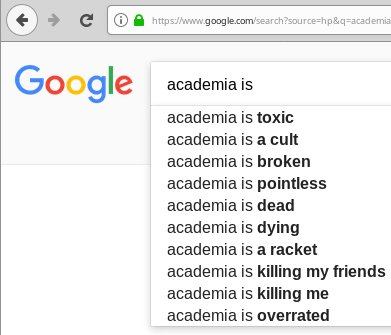
\includegraphics[width=.5\textwidth]{academia_is.png}
% \end{frame}

\end{document}

